\documentclass[a4, 12pt]{article}
\usepackage{booktabs, multirow}
\usepackage{soul}
\usepackage{xcolor,colortbl}
\usepackage{changepage,threeparttable}
\usepackage[english]{babel}
\usepackage[utf8]{inputenc}
\usepackage{graphicx}
\usepackage{fancyhdr}
\usepackage[hidelinks]{hyperref}
\usepackage{float}
\pagestyle{fancy}
\fancyhf{}
\lhead{Cornell University}
\rhead{\today}
\cfoot{\thepage}
\lfoot{Bryan Peters}
\rfoot{Sandia SAND: N/A}
\renewcommand{\headrulewidth}{0.5pt}
\renewcommand{\footrulewidth}{0.5pt}

\begin{document}

\begin{titlepage}

\begin{center}
   
\includegraphics[scale=1.6]{Images/bold_cornell_seal_pms187_red.eps} 
\end{center}
   
\thispagestyle{fancy}

\center

\textsc{\large M.Eng PROPOSAL}

\vspace{0.5in}

\noindent\makebox[\linewidth]{\rule{\linewidth}{1.2pt}}
\textsc{ \textbf{\large Test/Flight readiness development of ChipSats}}
\noindent\makebox[\linewidth]{\rule{\linewidth}{1.2pt}}

\vspace{0.5in}

\begin{minipage}{0.48\textwidth}
    \begin{flushleft}
        \textit{Student:} \\
        Bryan Peters \\
        Cornell University \\
        bmp85@cornell.edu
    \end{flushleft}
\end{minipage}
\begin{minipage}{0.48\textwidth}
    \begin{flushright}
    \textit{Advisor:} \\
    Dr.Joseph Skovira \\
    \textit{Out of Department Advisor:}\\
    Joshua Umansky-Castro\\
    \end{flushright}
\end{minipage}

\vspace{2in}

\textbf{\large Department of Electrical and Computer Engineering} \\

\thispagestyle{empty}
\end{titlepage}

\newpage


\tableofcontents
\newpage

%%%------------------------------------------------------------------------------------------
%%          Sections of the paper. All located in seperate files to improve readbility.
%%%------------------------------------------------------------------------------------------
\section{Background}
\par This project will focus on assisting the SSDS team with two different systems and a milestone test leading up to a spaceflight at some point in the future. The two systems are the alpha ChipSat, and the DeSCENT chip sattelites. The Alpha ChipSat is majorly completed -- final flight units are expected to be due in the very near future -- it is likely no major changes will be made. However, environemental testing still needs to be done on the flight units along with power and some reliability testing. These ChipSattelites will be the main communications interface on the light sail that CubeSat will be deploying. 

The DeSCENT mission is slightly different in comparison to the Alpha ChipSat. DeSCENT is the Demonstration of Suborbital Chipsats Ejected from New Shepard Test flight. Where the goal of this mission is to deploy a large number of chip satelites from Blue Origin's New Shepard launch vehicle. The New Shepard typically has an apogee of around 100-106km, just barely at the edge of space by international standards and well into space by U.S. standards.
After deploying these craft fall back down to earth, 
collecting and transmitting data like temperature, pressure, vehicle orientation etc the entire time.
Under ideal conditions these chipsats will be communicating their location to us once on the ground, allowing for at least one or two recoveries. However there are a lot of factors at play for that to happen out of one hundred we can likely hope for 3-4 to be recovered. 
\section{Tasks and Requirements}
\subsection{DeSCENT}

On the DeSCENT mission there is still a lot of work to be done over the year. There is significant amounts of work to be done on the power and RF side of the V1 chipsat We are just beginning the work of a new version of the DeSCENT chipsat 
%%%%%%%%%%%%%%%%%%%
durrently dubbed v2 - but hopefully changing to Tiberius.
%%%%%%%%%%%%%%%%%%%
On this new version some of the major work to be done is:
\begin{enumerate}
    \item WIO-E5 footprinting
    \item WIO-E5 PCB implementation
    \item Breadboarding to test WIO-E5 circuitry
    \item Testing of PCBs when they arrive
    \item Power testing and design \begin{enumerate}
        \item Falling weight balance
        \item Maple seed design
            \end{enumerate}
    \item Breadboarding and testing of both v1 and v2
\end{enumerate}
\begin{figure}[H]
    \begin{center}
            \includegraphics[width=.9\textwidth]{Images/Descent.jpg}\caption{Version one of the DeSCENT ChipSat.}
    \end{center}
\end{figure}

\subsection{Alpha ChipSat and Picoballoon}

As far as the Alpha ChipSat goes there is far less to do. Mainly involving finishing touches and testing the infrastructe that we are planning to use for communications once in space. The infrastructure test will be done using a high altitude balloon. Some goals for this part of the project are:
\begin{enumerate}
    \item Validate balloon test solar setup \begin{enumerate}
        \item Power is on and consistant throughout flight
        \item Longer duration than the last flight -- both signals dropped at 90ß minutes.
        \item Able to transmit consistently -- very power hungry
    \end{enumerate}
    \item Launch balloon test
    \item circumnavigate the globe with the high altitude balloon
    \item Solve GPS power up issue
\end{enumerate}
\begin{figure}[H]
    \begin{center}
            \includegraphics[width=.9\textwidth]{Images/Alpha.jpg}\caption{A current Alpha ChipSat.}
    \end{center}
\end{figure}
\section{Deliverables}
Given the short timeframe of a semester, and excluding a lot of work that is going to be done I have honed in on two main deliverables.
\begin{enumerate}
    \item 1-2 more PicoBalloon launches
    \item A fully tested and working V1 DeSCENT \begin{enumerate}
        \item Or a breadboarded and tested V2 chipsat
    \end{enumerate}
\end{enumerate}

While there will be plenty of work outside these deliverables taking place over the course of the semester, these are what I believe are good milestones. 
% \section{Methods}
During the course of this project I have been able to learn a significant amount about antenna tuning, new programming methods, and how the multilpe agencies that control spaceflight interact during the development phase of a launch.
First let's explore what progress has been made on the alpha chipsat as that was my main focus for the majority of the semester so far. A short list of whats been accomplished on alpha so far is:
\begin{enumerate}
    \item Solar Testing
        \begin{enumerate}
        \item Power regulation circuit capacitors
        \item Solar power characterization for the Balloon test
        \end{enumerate}
    \item v4.76 Chipsat assembly
        \begin{enumerate}
        \item Soldered all components
        \item Tested functionality and troubleshooted
        \item Discovered a major flaw with GPS and clock speed
        \end{enumerate}
    \item LightSail Antenna tuning
        \begin{enumerate}
        \item Assisted in tuning antennas on one Chipsat for the alpha lightsail
        \end{enumerate}
    \item GPS lock Testing
\end{enumerate}

Working with the solar system on the alpha chipsat was fairly straightforward, we have lights in the basement that match the solar panels peak frequency of around 850nm. The lights are setup to energize the solar panel with a short circuit current of around 100mA. This current should be ample to power the Chipsat throuhg boot up, though issues may occur on a transmission.
One round of this testing was done in Rhodes B40, using a specific light to make sure that the chipsats would function on solar power exclusively. This test showed overall very bad results, the EDU chipsat 
\textbf{INSERT PICTURE HERE}

\section{Timeline}
A timeline for this semester can be seen in figure 3 there are a significant amount of tasks that overlap. In some cases it could be seen that there are also very few tasks for november. Both of these observations are due to the fact that the PicoBalloon is highly affected by weather and the fact that future work on the PicoBalloon is based on how the second test goes in october, weather prevailing.
\begin{figure}[H]
    \begin{center}
            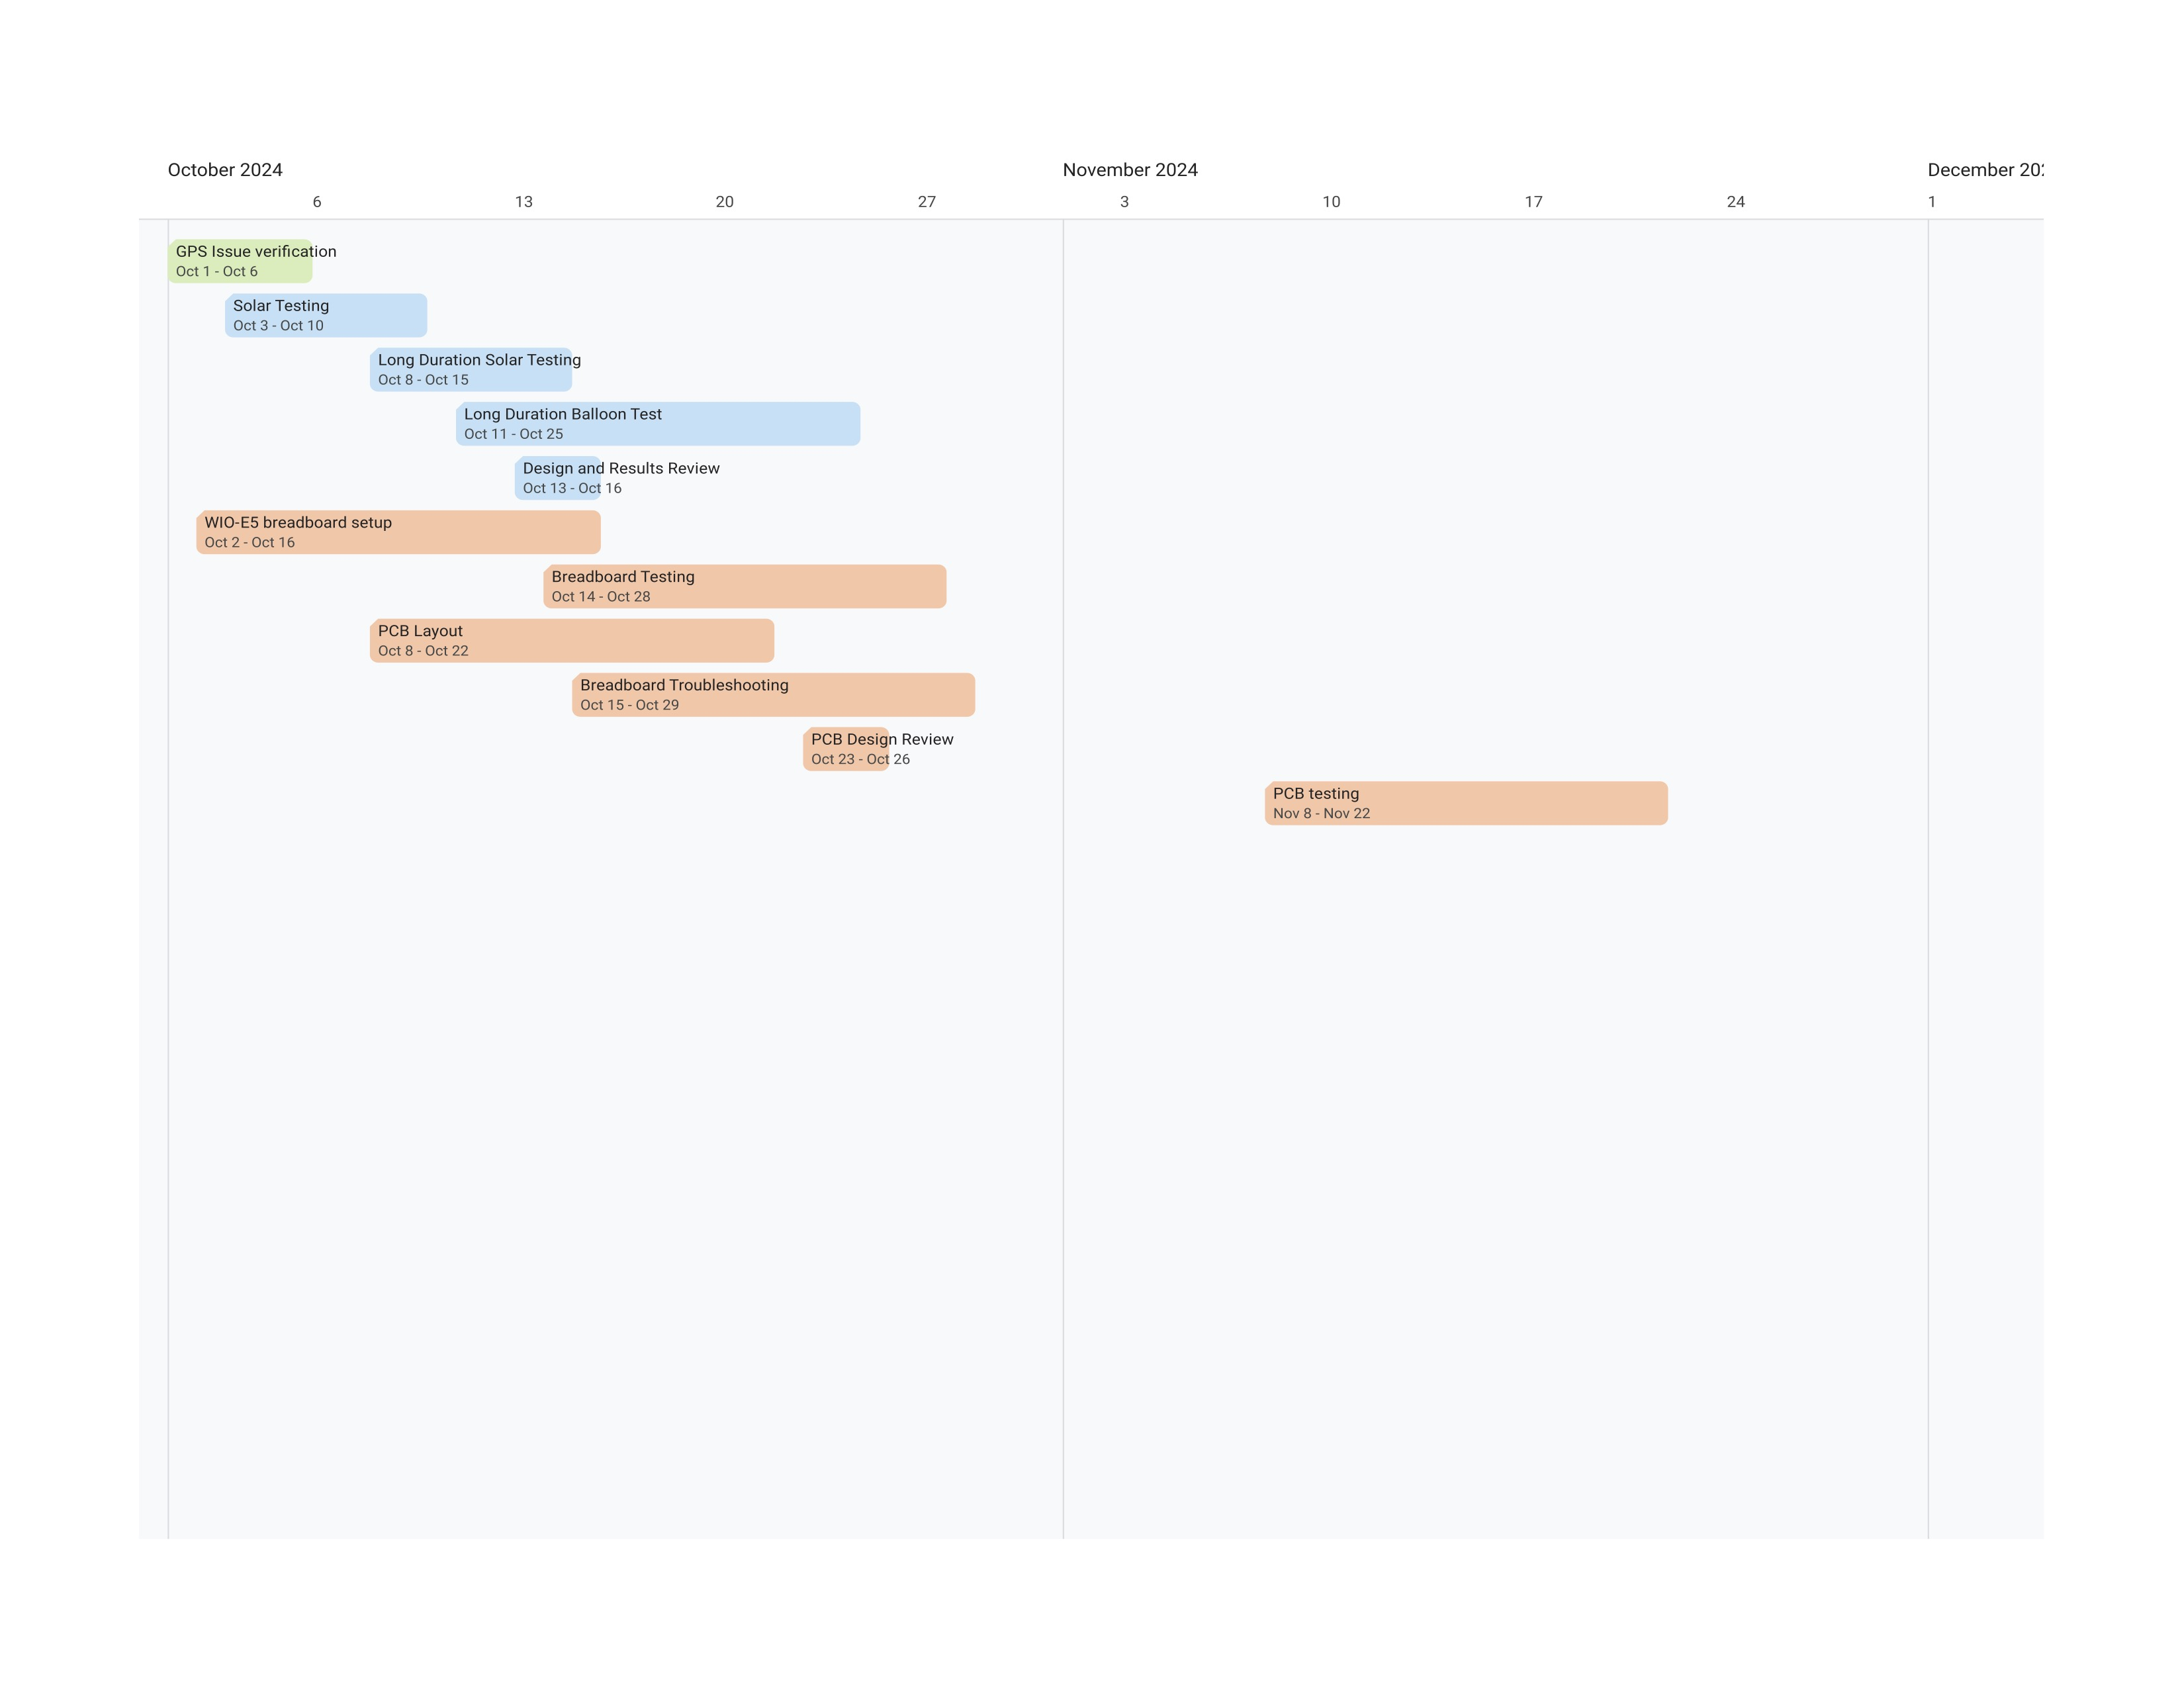
\includegraphics[width=1\textwidth]{Images/SSDS Timeline.jpg}\caption{A (mostly) semester long timeline for SSDS work}
    \end{center}
\end{figure}
The DeSCENT mission tasks are all in orange, these tasks are on a rolling timeline essentially as some of them are sequential, and V2 is not the main priority. The launch window could open as soon as november, so working out any issues with the V1 is crucial  before then. If the focus this semester becomes solely V1 then V2 will be the focus of next semester. Figure 3 is difficult to read so here is the data that went into the chart
\begin{table}[!htp]\centering
    \scriptsize
    \begin{tabular}{lrr}\toprule
        Task &Duration(days) \\\cmidrule{1-2}
        GPS Issue verification &5 \\
        Solar Testing &7 \\
        Long Duration Solar Testing &7 \\
        Long Duration Balloon Test &14 \\
        Design and Results Review &3 \\
        WIO-E5 breadboard setup &21 \\
        Breadboard Testing &21 \\
        PCB Layout &14 \\
        Breadboard Troubleshooting &21 \\
        PCB Design Review &3 \\
        PCB testing &14 \\
        \bottomrule
    \end{tabular}
\end{table}
Moving into the next semester will consist majorly of testing the V2 chipsat, which is beginning to be ordered as of now -- Nov 2024. Given that this project is research based I originally left out next semester from the timeline because it would be heavily based on what occured this semester. This semester has been filled with more issues than wins on the picoballoon chip sats and the v2 mcu, less progress than initially intended has been achieved. This actually works out well on a project basis as it leaves a significant amount of work for the V2 chipsat in semester 2.
\section{Conclusion}
Though time is extremely limited there is significant work and progress that can be made on both described systems, including the PicoBalloon project. With launches slated for next semester a majority of work must be completed this semester. Projects will continue into V2 or even new project opportunities next semester. With that being said this is a perfect opportunity for me to learn what goes into space systems design and learn the specific techniques used in this design space, all while providing my own expertise to the group.
%%%------------------------------------------------------------------------------------------

\bibliography{sources}
\bibliographystyle{IEEEtran}
\end{document}
